\documentclass[a4paper]{article}
\usepackage[utf8]{inputenc}
\usepackage[T1]{fontenc}
%\usepackage[french]{babel}
\usepackage{listings}
\usepackage{color}
\usepackage[usenames,dvipsnames,svgnames,table]{xcolor}
%\usepackage{titlesec}
\usepackage{tikz}
\usetikzlibrary{trees}
\usetikzlibrary{decorations.pathmorphing}
\usetikzlibrary{decorations.markings}


% Title Page
\title{SER - Labo4 \\}
\author{Yann Lederrey \& Joel Schär}


    \lstset{
    	tabsize=3,
    	inputencoding=utf8,
    	frame=lines,
    	caption=Test,
    	label=code:sample,
    	frame=shadowbox,
    	rulesepcolor=\color{gray},
    	xleftmargin=20pt,
    	framexleftmargin=15pt,
    	keywordstyle=\color{blue},
    	commentstyle=\color{OliveGreen},
    	stringstyle=\color{red},
    	numbers=left,
    	numberstyle=\scriptsize,
    	numbersep=5pt,
    	breaklines=true,
    	showstringspaces=false,
    	basicstyle=\footnotesize,
    	emph={cinema, projections, films, acteurs, motsCle, genres, langages, critiques },emphstyle={\color{magenta}}
    }
    
    \colorlet{punct}{red!60!black}
    \definecolor{delim}{RGB}{20,105,176}
    \colorlet{numb}{magenta!60!black}
    
    \lstdefinelanguage{json}{
    	stepnumber=1,
    	numbersep=5pt,
    	showstringspaces=false,
    	breaklines=true,
    	literate=
    	*{0}{{{\color{numb}0}}}{1}
    	{1}{{{\color{numb}1}}}{1}
    	{2}{{{\color{numb}2}}}{1}
    	{3}{{{\color{numb}3}}}{1}
    	{4}{{{\color{numb}4}}}{1}
    	{5}{{{\color{numb}5}}}{1}
    	{6}{{{\color{numb}6}}}{1}
    	{7}{{{\color{numb}7}}}{1}
    	{8}{{{\color{numb}8}}}{1}
    	{9}{{{\color{numb}9}}}{1}
    	{:}{{{\color{punct}{:}}}}{1}
    	{,}{{{\color{punct}{,}}}}{1}
    	{\{}{{{\color{delim}{\{}}}}{1}
    	{\}}{{{\color{delim}{\}}}}}{1}
    	{[}{{{\color{delim}{[}}}}{1}
    	{]}{{{\color{delim}{]}}}}{1},
    }
    
    
    \definecolor{amber}{rgb}{1.0, 0.49, 0.0}
    \definecolor{jaune}{rgb}{1.0, 0.75, 0.0}
    \definecolor{amethyst}{rgb}{0.6, 0.4, 0.8}
    \definecolor{antiquebrass}{rgb}{0.8, 0.58, 0.46}
    \definecolor{aqua}{rgb}{0.0, 1.0, 1.0}
    \definecolor{babypink}{rgb}{0.96, 0.76, 0.76}
   
   %delete first line indent
   \setlength{\parindent}{0in}
    
\begin{document}
\maketitle
\pagebreak

\tableofcontents
\pagebreak

\section{Introduction}
Ce rapport détailles les opérations demandé au laboratoire 4 de Sérialisation. Le but était d'échanger des informations entre plusieurs applicatifs en utilisant la méthode RMI.\\
Premièrement il fallait permettre l'échange de l'état actuel de la base de données entre l'application WFC (contenant la base de données) et l'application générale PlexAdmin.\\
Ensuite il fallait permettre à l'application PlexMedia de récupérer le fichier Json contenant la liste des projections cela en le demandant à PlexAdmin.


\section{Fonctionnement Générale}
Ici je vais vous expliquer le fonctionnement générale et l'interaction entre les applications dans le cadre du laboratoire 4. Seulement des actions en rapport avec le laboratoire 4 seront montrées.\\
Premièrement il faut savoir qu'il est nécessaire de démarrer les applicatifs dans l'ordre suivant:\\
\begin{itemize}
 \item WFC
 \item PlexAdmin
 \item PlexMedia
\end{itemize}
L'ordre doit être respecté car certaines application ont un rôle de serveur RMI ou Client ou les deux et bien-sur les serveurs doivent être démarré avant leur client respectif.\\

Aucun fichier Json/Xml n'ont étés modifiés, seulement les fichier java on été modifiés.

\subsection{WFC}
Le seul but de WFC et d'aller récupérer des données dans un base de données se trouvant à l'HEIG-VD et de retransmettre ces informations à PlexAdmin. Afin d'effectuer au mieux la transmission d'informations. PlexAdmin est observateur de WFC. C'est à dire que lorsque 
WFC annonce un changement (il a récupéré de nouvelles informations provenant de la base de données) il va alors notifier PlexAdmin pour que celui-ci invoque un update des données qui transite entre les deux applications.\\

\subsubsection{Conception}
Les classes modifiées sur WFC sont les suivantes :
\begin{itemize}
 \item Main.java
\end{itemize}

Le code des classes modifiées ont été rendues avec le rapport.\\

Si je résume ce qu'il se passe dans les main par rapport à RMI : 
\begin{itemize}
 \item Premièrement je crée un Registry sur le port 9999, le crée un service et je le bind avec le nom ``RmiService''.
 \item Ensuite dans le méthode Run qui va tourner en fond j'ajoute les méthodes permettant de signaler une mise à jour des données via
 setChanged et notifyObservers.
 \item j'implémente les méthodes nécessaires au modèle Observer/Observé et à la mise à jour des informations.
\end{itemize}

Pour résumé lorsque PlexAdmin se connecte il communique à WFC son existence, celui-ci va alors l'ajouter dans sa liste d'observable.\\
Ensuite lorsque WFC notifie PlexAdmin d'une mise à jour ce dernier va invoquer la méthode partagée getData afin de récupérer les données.


\subsection{PlexAdmin}
Pour ce laboratoire PlexAdmin a le rôle de récupérer les informations en provenance de WFC et de mettre à jour ça liste de films etc...\\
Après avoir définis une liste de projections, et généré un Json contenant cette liste, PlexAdmin doit permettre au client PlexMedia de récupérer ce fichier Json via RMI.\\

\subsubsection{Conception}
Les classes modifiées sur PlexAdmin sont les suivantes :
\begin{itemize}
 \item ControleurGeneral.java
 \item ControleurWFC.java
 \item ControleurMedia.java
 \item WFC-Interface/rmi/IserverMediaApi
\end{itemize}

Le code des classes modifiées ont été rendues avec le rapport.\\

Si je résume ce qu'il se passe pour la partie WFC-PlexAdmin.\\
Ici PlexAdmin doit recevoir la notification de WFC lorsque celui-ci a mise à jour ses informations, récupérer les nouvelles données puis mettre à jour ses propres informations.
\begin{itemize}
 \item Premièrement dans le ControleurGeneral je vais définir quel serveur RMI PlexAdmin doit écouter. Pour cela je définis un remoteService sur le port 9999
 en localhost/RmiService.
 \item Ensuite dans la classe ControleurWFC je définis les méthodes nécessaires au modèle Observer/Observé ainsi que 
 les méthodes des Interface.
\end{itemize}

Si je résume ce qu'il se passe pour la partie PlexAdmin-PlexMedia.\\
Ici PlexAdmin prend le rôle de serveur et PlexMedia de client. PlexAdmin doit alors fournir à PlexMedia la méthode nécessaire à récupérer un payload json de projections.
\begin{itemize}
 \item Premièrement dans le ControleurMedia je vais définir le serveur RMI en créant une nouvelle registrie sur le port 9998.
 que je bind sur ``Rmimedia``.
 \item Ensuite je définis les méthodes nécessaires au modèle Observer/Observé et les méthodes des Interface en communs permettant la récupération des informations.
 \item la méthode sendJSONToMedia crée le Json et notifie PlexMedia que celui-ci a été mis à jour. La méthode getData permet de récupérer le Json en format String.
\end{itemize}

Pour résumé lorsque PlexAdmin se connecte il communique à WFC son existence et démarre un thread ``startCheckingThread'' qui va vérifier continuellement que le serveur est joignable
WFC va ensuite l'ajouter dans sa liste d'observable. Lorsque la connexion est initialisée PlexAdmin demande son ajout dans les Observable. Lorsque PlexAdmin reçoit un signal (une notification) il demande à récupérer les données et met à jour ses informations. (méthode update).

Ensuite lorsque PlexAdmin a crée une liste de projections et généré le Json cela notifie PlexMedia qui peut alors mettre à jour ça liste en appelant la méthode commune getData et reçoit alors un payload Json en format String contenant les projections.

\subsection{PlexMedia}
PlexMedia a pour but de récupérer un Json contenant la liste des projections depuis PlexAdmin, Pour cela un bouton update a été crée permettant de faire cette récupération.

\subsubsection{Conception}
Les classes modifiées sur WFC sont les suivantes :
\begin{itemize}
 \item Amorce.java
 \item mainController
 \item WFC-Interface/rmi/IserverMediaApi
\end{itemize}

Le code des classes modifiées ont été rendues avec le rapport.\\

Si je résume ce qu'il se passe pour PlexMedia : 
\begin{itemize}
 \item Premièrement dans l'Amorce je démarre l'Interface graphique et par la mémé occasion le mainController.
 \item Ensuite dans la méthode initialize du mainController je mets en écoute PlexMedia sur le port 9998 en localhost/Rmimedia
 \item Puis finalement j'implémente et utilise les méthode permettant de récupérer le fichier Json à travers RMI.
\end{itemize}

Pour résumer lorsque l'on clique sur le bouton update PlexMedia va invoquer la méthode commune provenant de l'Interface IserverMediaApi permettant de récupérer le payload Json de PlexAdmin.
Puis va afficher son contenant en terminal.


\subsection{Utilisation}

\begin{itemize}
 \item État de PlexAdmin avant la mise à jour de ses données :\\ 
 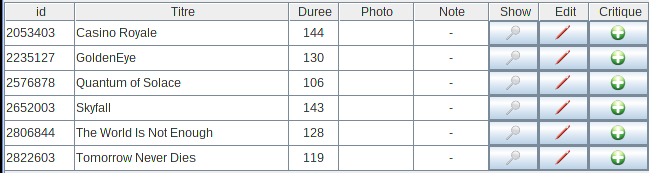
\includegraphics[scale=0.5]{beforeUpdate.png}
 \item Mise a jour des données sur WFC : \\ 
 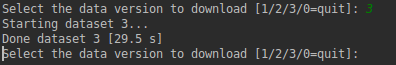
\includegraphics[scale=0.5]{updateDatabase.png}
 \item État de PlexAdmin après la mise à jour des données :\\ 
 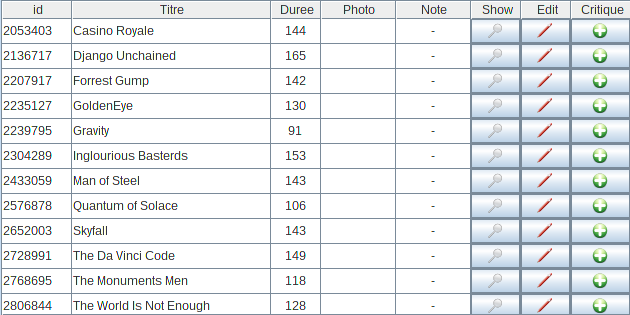
\includegraphics[scale=0.5]{AfterUpdate.png}
 \item Création de projections sur PlexAdmin :\\ 
 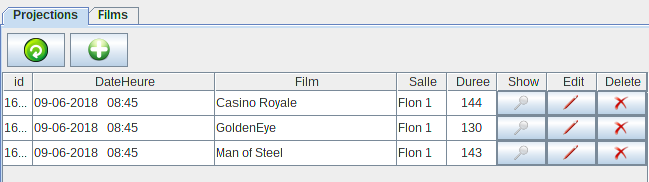
\includegraphics[scale=0.5]{SelectProjection.png}
 \item Création du fichier Json sur PlexAdmin :\\ 
 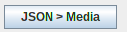
\includegraphics[scale=0.5]{CreateJson.png}
 \item demande de mise à jour sur PlexMedia :\\ 
 
\includegraphics[scale=0.5]{updatePlexMedia.png}
 \item nouveau payload Json pour PlexMedia :\\ 
 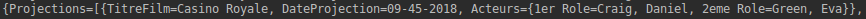
\includegraphics[scale=0.5]{PayloadJson.png}
\end{itemize}

\section{conclusion}
Ce laboratoire a été intéressant et nous a fait découvrir une nouvelle technologie. Je ne suis pas sur de souvent réutiliser RMI mais il est toujours instructif de connaître de nouvelle

\end{document}          
	